\documentclass{article}
\usepackage[margin=1in]{geometry}
\usepackage{amsmath}
\usepackage{amsfonts}
\usepackage{graphicx}
\usepackage{xcolor}
\usepackage{ulem}
% Calligraphic fonts
\newcommand{\calA}{{\cal A}}
\newcommand{\calB}{{\cal B}}
\newcommand{\calC}{{\cal C}}
\newcommand{\calD}{{\cal D}}
\newcommand{\calE}{{\cal E}}
\newcommand{\calF}{{\cal F}}
\newcommand{\calG}{{\cal G}}
\newcommand{\calH}{{\cal H}}
\newcommand{\calI}{{\cal I}}
\newcommand{\calJ}{{\cal J}}
\newcommand{\calK}{{\cal K}}
\newcommand{\calL}{{\cal L}}
\newcommand{\calM}{{\cal M}}
\newcommand{\calN}{{\cal N}}
\newcommand{\calO}{{\cal O}}
\newcommand{\calP}{{\cal P}}
\newcommand{\calQ}{{\cal Q}}
\newcommand{\calR}{{\cal R}}
\newcommand{\calS}{{\cal S}}
\newcommand{\calT}{{\cal T}}
\newcommand{\calU}{{\cal U}}
\newcommand{\calV}{{\cal V}}
\newcommand{\calW}{{\cal W}}
\newcommand{\calX}{{\cal X}}
\newcommand{\calY}{{\cal Y}}
\newcommand{\calZ}{{\cal Z}}

% Sets:
\newcommand{\setA}{\textsf{A}}
\newcommand{\setB}{\textsf{B}}
\newcommand{\setC}{\textsf{C}}
\newcommand{\setD}{\textsf{D}}
\newcommand{\setE}{\textsf{E}}
\newcommand{\setF}{\textsf{F}}
\newcommand{\setG}{\textsf{G}}
\newcommand{\setH}{\textsf{H}}
\newcommand{\setI}{\textsf{I}}
\newcommand{\setJ}{\textsf{J}}
\newcommand{\setK}{\textsf{K}}
\newcommand{\setL}{\textsf{L}}
\newcommand{\setM}{\textsf{M}}
\newcommand{\setN}{\textsf{N}}
\newcommand{\setO}{\textsf{O}}
\newcommand{\setP}{\textsf{P}}
\newcommand{\setQ}{\textsf{Q}}
\newcommand{\setR}{\textsf{R}}
\newcommand{\setS}{\textsf{S}}
\newcommand{\setT}{\textsf{T}}
\newcommand{\setU}{\textsf{U}}
\newcommand{\setV}{\textsf{V}}
\newcommand{\setW}{\textsf{W}}
\newcommand{\setX}{\textsf{X}}
\newcommand{\setY}{\textsf{Y}}
\newcommand{\setZ}{\textsf{Z}}

% Vectors
\newcommand{\bfa}{\mathbf{a}}
\newcommand{\bfb}{\mathbf{b}}
\newcommand{\bfc}{\mathbf{c}}
\newcommand{\bfd}{\mathbf{d}}
\newcommand{\bfe}{\mathbf{e}}
\newcommand{\bff}{\mathbf{f}}
\newcommand{\bfg}{\mathbf{g}}
\newcommand{\bfh}{\mathbf{h}}
\newcommand{\bfi}{\mathbf{i}}
\newcommand{\bfj}{\mathbf{j}}
\newcommand{\bfk}{\mathbf{k}}
\newcommand{\bfl}{\mathbf{l}}
\newcommand{\bfm}{\mathbf{m}}
\newcommand{\bfn}{\mathbf{n}}
\newcommand{\bfo}{\mathbf{o}}
\newcommand{\bfp}{\mathbf{p}}
\newcommand{\bfq}{\mathbf{q}}
\newcommand{\bfr}{\mathbf{r}}
\newcommand{\bfs}{\mathbf{s}}
\newcommand{\bft}{\mathbf{t}}
\newcommand{\bfu}{\mathbf{u}}
\newcommand{\bfv}{\mathbf{v}}
\newcommand{\bfw}{\mathbf{w}}
\newcommand{\bfx}{\mathbf{x}}
\newcommand{\bfy}{\mathbf{y}}
\newcommand{\bfz}{\mathbf{z}}


\newcommand{\bfalpha}{\boldsymbol{\alpha}}
\newcommand{\bfbeta}{\boldsymbol{\beta}}
\newcommand{\bfgamma}{\boldsymbol{\gamma}}
\newcommand{\bfdelta}{\boldsymbol{\delta}}
\newcommand{\bfepsilon}{\boldsymbol{\epsilon}}
\newcommand{\bfzeta}{\boldsymbol{\zeta}}
\newcommand{\bfeta}{\boldsymbol{\eta}}
\newcommand{\bftheta}{\boldsymbol{\theta}}
\newcommand{\bfiota}{\boldsymbol{\iota}}
\newcommand{\bfkappa}{\boldsymbol{\kappa}}
\newcommand{\bflambda}{\boldsymbol{\lambda}}
\newcommand{\bfmu}{\boldsymbol{\mu}}
\newcommand{\bfnu}{\boldsymbol{\nu}}
\newcommand{\bfomicron}{\boldsymbol{\omicron}}
\newcommand{\bfpi}{\boldsymbol{\pi}}
\newcommand{\bfrho}{\boldsymbol{\rho}}
\newcommand{\bfsigma}{\boldsymbol{\sigma}}
\newcommand{\bftau}{\boldsymbol{\tau}}
\newcommand{\bfupsilon}{\boldsymbol{\upsilon}}
\newcommand{\bfphi}{\boldsymbol{\phi}}
\newcommand{\bfchi}{\boldsymbol{\chi}}
\newcommand{\bfpsi}{\boldsymbol{\psi}}
\newcommand{\bfomega}{\boldsymbol{\omega}}
\newcommand{\bfxi}{\boldsymbol{\xi}}
\newcommand{\bfell}{\boldsymbol{\ell}}

% Matrices
\newcommand{\bfA}{\mathbf{A}}
\newcommand{\bfB}{\mathbf{B}}
\newcommand{\bfC}{\mathbf{C}}
\newcommand{\bfD}{\mathbf{D}}
\newcommand{\bfE}{\mathbf{E}}
\newcommand{\bfF}{\mathbf{F}}
\newcommand{\bfG}{\mathbf{G}}
\newcommand{\bfH}{\mathbf{H}}
\newcommand{\bfI}{\mathbf{I}}
\newcommand{\bfJ}{\mathbf{J}}
\newcommand{\bfK}{\mathbf{K}}
\newcommand{\bfL}{\mathbf{L}}
\newcommand{\bfM}{\mathbf{M}}
\newcommand{\bfN}{\mathbf{N}}
\newcommand{\bfO}{\mathbf{O}}
\newcommand{\bfP}{\mathbf{P}}
\newcommand{\bfQ}{\mathbf{Q}}
\newcommand{\bfR}{\mathbf{R}}
\newcommand{\bfS}{\mathbf{S}}
\newcommand{\bfT}{\mathbf{T}}
\newcommand{\bfU}{\mathbf{U}}
\newcommand{\bfV}{\mathbf{V}}
\newcommand{\bfW}{\mathbf{W}}
\newcommand{\bfX}{\mathbf{X}}
\newcommand{\bfY}{\mathbf{Y}}
\newcommand{\bfZ}{\mathbf{Z}}


\newcommand{\bfGamma}{\boldsymbol{\Gamma}}
\newcommand{\bfDelta}{\boldsymbol{\Delta}}
\newcommand{\bfTheta}{\boldsymbol{\Theta}}
\newcommand{\bfLambda}{\boldsymbol{\Lambda}}
\newcommand{\bfPi}{\boldsymbol{\Pi}}
\newcommand{\bfSigma}{\boldsymbol{\Sigma}}
\newcommand{\bfUpsilon}{\boldsymbol{\Upsilon}}
\newcommand{\bfPhi}{\boldsymbol{\Phi}}
\newcommand{\bfPsi}{\boldsymbol{\Psi}}
\newcommand{\bfOmega}{\boldsymbol{\Omega}}


% Blackboard Bold:
\newcommand{\bbA}{\mathbb{A}}
\newcommand{\bbB}{\mathbb{B}}
\newcommand{\bbC}{\mathbb{C}}
\newcommand{\bbD}{\mathbb{D}}
\newcommand{\bbE}{\mathbb{E}}
\newcommand{\bbF}{\mathbb{F}}
\newcommand{\bbG}{\mathbb{G}}
\newcommand{\bbH}{\mathbb{H}}
\newcommand{\bbI}{\mathbb{I}}
\newcommand{\bbJ}{\mathbb{J}}
\newcommand{\bbK}{\mathbb{K}}
\newcommand{\bbL}{\mathbb{L}}
\newcommand{\bbM}{\mathbb{M}}
\newcommand{\bbN}{\mathbb{N}}
\newcommand{\bbO}{\mathbb{O}}
\newcommand{\bbP}{\mathbb{P}}
\newcommand{\bbQ}{\mathbb{Q}}
\newcommand{\bbR}{\mathbb{R}}
\newcommand{\bbS}{\mathbb{S}}
\newcommand{\bbT}{\mathbb{T}}
\newcommand{\bbU}{\mathbb{U}}
\newcommand{\bbV}{\mathbb{V}}
\newcommand{\bbW}{\mathbb{W}}
\newcommand{\bbX}{\mathbb{X}}
\newcommand{\bbY}{\mathbb{Y}}
\newcommand{\bbZ}{\mathbb{Z}}






\title{ECE 498/598 Midterm 2 2023}
\date{Nov 8th, 2023}
\author{Instructor: Vikas Dhiman}

\newtheorem{prob}{Problem}
\newif\ifsol
\solfalse

\begin{document}
\maketitle
%$ \hat{\mathbf{w}} = \hat{\mathbf{k}} \times \frac{\mathbf{v}}{\|\mathbf{v}\|} $
%$ \|\hat{\mathbf{w}}\| = \|\hat{\mathbf{k}}\| \|\frac{\mathbf{v}}{\|\mathbf{v}\|}\| \sin(\phi) $. 

\begin{tabular}{p{0.5\linewidth}p{0.5\linewidth}}
  (1) Student name:& Student email: \\
\end{tabular}

\subsubsection*{About the exam}
\begin{enumerate}
  \item There are total 4 problems. You must attempt all 4.
  \item Maximum marks: 50.
  \item Maximum time allotted:  50 min
  \item Calculators are allowed.
  \item One US Letter size or A4 size cheat sheet (both-sides) is allowed.
\end{enumerate}

\begin{prob}
  Find the 4x4 transformation matrix $^1T_0$ that transforms coordinates from coordinate frame 1 to coordinate frame 0 (5 marks).\\
  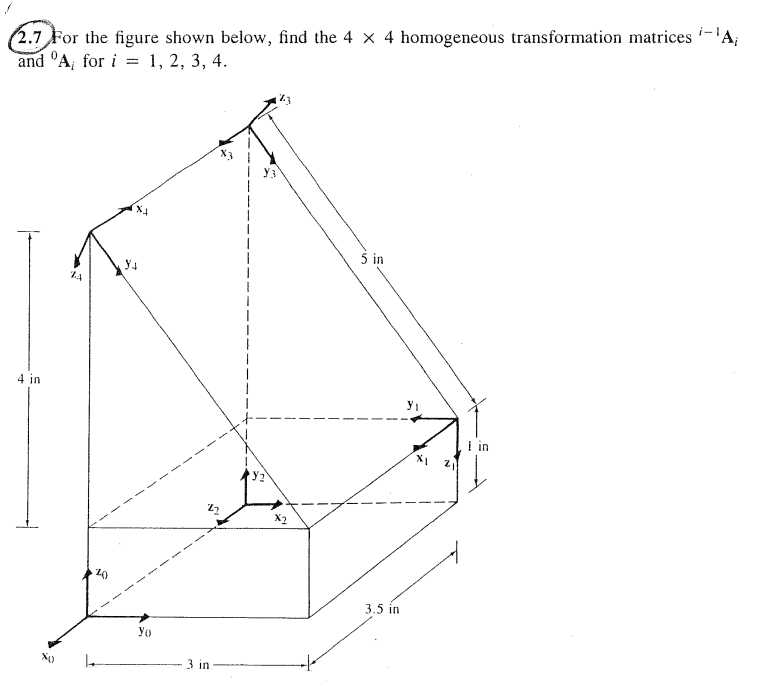
\includegraphics[width=0.7\linewidth,trim=0 0 0 1in,clip]{./media/transformations.png}
\end{prob}
I am going to write transform from frame 1 to frame 0. $^0T_1$
\begin{align}
  ^0T_1 = \begin{bmatrix}
    1 & 0 & 0 & -3.5\\
    0 & -1 & 0 & 3 \\
    0 & 0 & -1 & 1\\
    0 & 0 & 0 & 1
  \end{bmatrix}
\end{align}
The rotation matrix is obtained by writing the basis vectors of the destination coordinate system in the source coordinate system.

\newpage
.
\newpage

\begin{prob}
  Consider a coordinate system OUVW whose ordered set of basis vectors given by
  $\bfu = [3/7, 2/7, 6/7]^\top$, $\bfv = [2/7, 6/7, 3/7]^\top$ and $\bfw = [4,
  5, 6]^\top$.
  Another coordinate system OXYZ whose order set of basis vectors is, $\bfx =
  [2/7, 6/7, -3/7]^\top$, $\bfy = [-6/7, 3/7, 2/7]^\top$ and $\bfz = [3/7, 2/7, 6/7]^\top$.
  Find the rotation matrix $^{ouvw}R_{oxyz}$ that converts coordinates from frame OXYZ to frame OUVW. (10 marks)
\end{prob}
\begin{align}
  ^{OUVW}R_{OPQR} &= \begin{bmatrix}
    3/7 & 2/7 & 4 \\
    2/7 & 6/7 & 5  \\
    6/7 & 3/7 & 6 \\
  \end{bmatrix} \\
  ^{OXYZ}R_{OPQR} &= \begin{bmatrix}
    2/7 & -6/7 & 3/7 \\
    6/7 & 3/7 & 2/7  \\
    -3/7 & 2/7 & 6/7 \\
  \end{bmatrix} \\
  ^{OUVW}R_{OXYZ} &= ^{OUVW}R_{OPQR} (^{OXYZ}R_{OPQR})^\top \\
&= \begin{bmatrix}
    3/7 & 2/7 & 4 \\
    2/7 & 6/7 & 5  \\
    6/7 & 3/7 & 6 \\
  \end{bmatrix}
\begin{bmatrix}
    2/7 & -6/7 & 3/7 \\
    6/7 & 3/7 & 2/7  \\
    -3/7 & 2/7 & 6/7 \\
  \end{bmatrix}^\top
\end{align}
\newpage

\begin{prob}
  (Rodrigues formula) In the figure below, we are rotating point $\bfv$ around
  axis unit-vector $\hat{\bfk}$ by an angle $\theta$. A unit vector $\hat{\bfw}$ is
  perpendicular to the both $\bfv$ and $\hat{\bfk}$. Another vector $\bfv_{\perp}$ is the projection of $\bfv$ onto a plane that is perpendicular to $\hat{\bfk}$. Note that $\bfv_{\perp}$ is perpendicular to both $\hat{\bfw}$ and $\hat{\bfk}$. First, (a) write the
  unit-vector $\hat{\bfw}$ in terms of $\bfv$ and $\hat{\bfk}$.
  (b) Then write the vector (including the correct magnitude) $\bfv_\perp$ in terms of $\bfv$ and $\hat{\bfk}$.
  (c) A vector $\bfv_{\perp,\text{rot}}$ is obtained by rotating $\bfv_\perp$ by an angle $\theta$. Write the vector $\bfv_{\perp,\text{rot}}$ in terms of $\bfv_{\perp}$, $\hat{\bfw}$ and $\theta$. 
  (15 marks)\\
  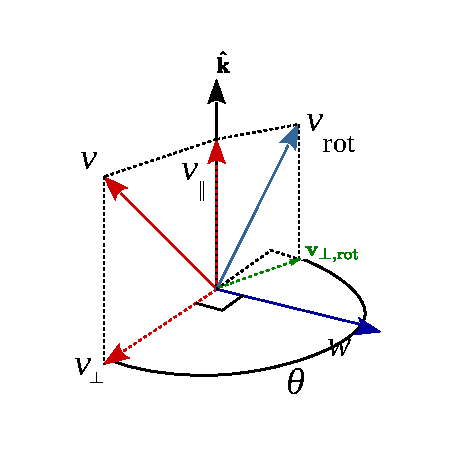
\includegraphics[width=0.5\linewidth]{media/Rodrigues-formula.pdf}
\end{prob}
\begin{align}
  \hat{\bfw} = \frac{\hat{\bfk} \times \bfv}{\|\hat{\bfk} \times \bfv\|}
\end{align}
Note that $\hat{\bfk} \times \bfv$ has the magnitude $\|\hat{\bfk} \times \bfv\| = |\hat{\bfk}||\bfv| \sin(\alpha) = |\bfv| \sin(\alpha)$ where $\alpha$ is the angle between $\bfv$ and $\hat{\bfk}$.
\begin{align}
\bfv_\perp = -\hat{\bfk} \times (\hat{\bfk} \times \bfv)
\end{align}
The magnitude of $\bfv_\perp$ is same as RHS because both $|\bfv_\perp| = |\bfv|\sin(\alpha)$ and $|-\hat{\bfk} \times (\hat{\bfk}  \times \bfv)| = |\bfv||\hat{\bfk}|^2 \sin(\alpha) \sin(90^\circ) = |\bfv|\sin(\alpha)$ where $\alpha$ is the angle between $\bfv$ and $\hat{\bfk}$.
\begin{align}
  \bfv_{\perp,rot} = \bfv_\perp \cos(\theta) +
  \hat{\bfw}|\hat{\bfk} \times \bfv| \sin(\theta)
\end{align}


\newpage

\begin{prob}
  The Euler angles of rotation YZX are given as $\theta$, $\phi$ and $\psi$.
  Derive the rotation matrix corresponding to the Euler angle representation $R = R_x(\psi) R_z(\phi) R_y(\theta)$. Also derive an expression to convert the rotation matrix back to Euler angles. (20 marks).
\end{prob}
\begin{align}
  R = R_x(\psi) R_z(\phi) R_y(\theta)
\end{align}
\begin{align}
  \implies \begin{bmatrix}
    r_{11} & r_{12} & r_{13}  \\
    r_{21} & r_{22} & r_{23}  \\
    r_{31} & r_{32} & r_{33}  
  \end{bmatrix}
  =
  \begin{bmatrix}
    1 & 0 & 0\\
    0 & c_\psi & -s_\psi \\
    0 & s_\psi & c_\psi \\
  \end{bmatrix}
  \begin{bmatrix}
    c_\phi & -s_\phi & 0 \\
    s_\phi & c_\phi & 0 \\
    0 & 0 & 1\\
  \end{bmatrix}
  \begin{bmatrix}
    c_\theta & 0 & s_\theta \\
    0 & 1 & 0\\
    -s_\theta & 0 & c_\theta \\
  \end{bmatrix}
\end{align}
\begin{align}
  = \begin{bmatrix}
    1 & 0 & 0\\
    0 & c_\psi & -s_\psi \\
    0 & s_\psi & c_\psi \\
  \end{bmatrix}
  \begin{bmatrix}
    c_\phi c_\theta & - s_\phi & c_\phi s_\theta \\
    s_\phi c_\theta &   c_\phi & s_\phi s_\theta \\
    -s_\theta & 0 & c_\theta \\
  \end{bmatrix}
\end{align}
\begin{align}
  \implies \begin{bmatrix}
    r_{11} & r_{12} & r_{13}  \\
    r_{21} & r_{22} & r_{23}  \\
    r_{31} & r_{32} & r_{33}  
  \end{bmatrix}
  = \begin{bmatrix}
    c_\phi c_\theta & - s_\phi & c_\phi s_\theta \\
    c_\psi s_\phi c_\theta + s_\psi s_\theta &  c_\psi c_\phi & c_\psi s_\phi s_\theta  - s_\psi c_\theta \\
    s_\psi s_\phi c_\theta - c_\psi s_\theta & s_\psi c_\phi & s_\psi s_\phi s_\theta + c_\psi c_\theta
  \end{bmatrix}
\end{align}

\begin{align}
  \phi &= \sin^{-1}(-r_{12}) \in [-\pi/2, \pi/2]\\
  \theta &= \text{arctan2}(r_{13}, r_{11}) \\
  \psi &= \text{arctan2}(r_{32}, r_{22})
\end{align}
\newpage

\end{document}
